\section{Synthesis Details and Artifact Checks}
\label[appendix]{app:artifact}

This appendix provides the search procedure, model encodings, and
additional checks underlying \Cref{tab:synthesis-results}.

\subsection{Search Procedure and Supplied Partitions}
\label[appendix]{app:synthesis-search}

Before searching, Z3 checks initial inclusion in $S$ and preservation
by each represented outcome. For an abstraction it also checks
$S\land b\Rightarrow\exists\xi\,A(\sigma,\xi)$, so every enabled
state admits an outcome description. This last query may be quantified.

Fix a coefficient bound $B$. Each unknown coefficient is an integer
between $-B$ and $B$. The search proceeds as follows:
\begin{enumerate}
 \item \emph{Choose a sample.} Z3 selects an enabled state in $S$
 and, if needed, an admissible $\xi$. If none exists, all initial
 states are already terminal.
 \item \emph{Propose coefficients.} The learner chooses both vectors
 so that all verification conditions hold on the accumulated samples.
 It minimizes the sum of absolute coefficient values to favor small
 expressions; this objective has no soundness role.
 \item \emph{Check all states.} With coefficients fixed, the verifier
 searches for an enabled state and admissible $\xi$ violating a condition.
 A counterexample is added to the samples before returning to the learner.
 \item \emph{Accept a verified pair.} An unsatisfiable verifier query
 establishes the conditions over the entire invariant domain, including
 unbounded integer inputs. The implementation accepts the pair after
 also checking each condition separately.
\end{enumerate}
The learner and verifier alternate which quantities are fixed.
On a fixed sample, the constraints are linear in the unknown template
coefficients. With coefficients fixed, they are Boolean combinations
of linear arithmetic in the state and auxiliary transition variables
for the supported encodings. The verification domain is never bounded
by the coefficient bound $B$.

Each counterexample excludes the current candidate and no valid one.
Thus exact terminating solvers, without resource limits, decide existence
within each finite coefficient set. The implementation tries
$B=1,2,4,8,16$, retaining samples between bounds. Learner unsatisfiability
excludes only the current bound; exhausting the schedule excludes only
the tested coefficient sets. Unknown results, timeouts, and the limit of 500
candidates are inconclusive and retain the available search context.
Relative completeness of the rule does not imply completeness of this
search: templates, domination, and a possibly overapproximating supplied
invariant can each exclude otherwise available certificates.

\paragraph{Fixed piecewise affine templates.}
The same procedure accepts a supplied finite partition
$P_1,\ldots,P_q$ of the enabled states in $S$.
It checks that the regions cover this domain and are pairwise disjoint,
then creates a separate affine coefficient block for each region and
each certificate. For example, the supermartingale template is
\[
 V(\sigma)=[b](\sigma)\sum_{j=1}^{q}[P_j](\sigma)
 \left(a_{j,0}+\sum_{i=1}^{d}a_{j,i}x_i(\sigma)\right).
\]
The variant template has its own coefficient blocks.
The partition predicates are supplied Boolean combinations of linear
arithmetic over declared state components, including symbolic program
inputs. They cannot depend on template coefficients or auxiliary
transition variables. The verifier evaluates the partition again at
each successor, so it also checks transitions between regions.
The verification conditions and their soundness argument are unchanged.

The algorithm searches for coefficients, not partition predicates or
thresholds. The two-sided walk in \Cref{app:synthesis-models} illustrates their
benefit; \Cref{app:synthesis-checks} gives optional sampler splits.

\subsection{Loop Models and Certificate Analysis}
\label[appendix]{app:synthesis-models}

The following models instantiate the common interface of
\Cref{sec:synthesis-constraints}. All displayed certificate expressions
are their values on enabled states; guarded templates assign zero on
terminal states.

\paragraph{Unbounded symmetric random walk.}
For the random walk in \Cref{sec:rule-examples}, the model has $S\equiv x\geq0$, guard
$x>0$, and the equally likely updates $x\mapsto x-1$ and $x\mapsto x+1$.
The engine constructs the basis $(x,1)$ and finds $V=U=x$ on enabled
states, verified without an upper bound on $x$. The expectation is
unchanged, while the left outcome decreases $U$ by one.
This establishes AST despite infinite expected runtime:
for $0<x<N$, the expected time $x(N-x)$ to hit $\{0,N\}$ lower-bounds
the expected time to hit $0$, and diverges with $N$.
A uniform negative expected drift is unnecessary.

\paragraph{FDR with a symbolic range.}
For the loop of \Cref{sec:fdr}, the supplied invariant is
$S\equiv n\geq1\land1\leq v<2n\land0\leq c<v\land c<n$, and the
complete bit-$\beta$ update is
\[
 T_\beta(n,v,c)=
 \begin{cases}
 (n,2v-n,2c+\beta-n),&2c+\beta\geq n,\\
 (n,2v,2c+\beta),&2c+\beta<n.
 \end{cases}
\]
Here $n$ is a read-only program input. From the declared integer
components the engine constructs the full basis $(n,v,c,1)$ and finds
$V=n$, $U=n-v+c$ on $v<n$, verified for all admitted values of $n$.
This recovers the affine certificates of \Cref{thm:fdr}.
Writing $\Delta=v-c\geq1$, the identity $\Delta'=2\Delta-\beta$
also yields $\mathbb E[U']\leq U-1/2$: bit zero decreases $U$ by
at least one, and bit one does not increase it; acceptance sets it to zero.
This stronger inequality is independently SMT-verified, so $U$ is itself
a ranking supermartingale.

\paragraph{FLDR with fixed weights.}
For $(4,5)$, preprocessing gives $m=9$, $k=4$, and rejection weight $7$.
The artifact constructs the exact tree using the row convention of
\Cref{sec:fldr}. Its loop-head nodes form the invariant, internal nodes
satisfy the guard, and the bit edges include resets. Since $m,k,n$ are
fixed numerical values, the integer state components are $c,d$, giving
the basis $(c,d,1)$. After excluding $B=1$, it finds
$V=U=c-2d+2$ at $B=2$. \Cref{fig:fldr-synthesis-tree} displays the
five active nodes, acceptances, and resets. An independent rational-arithmetic
audit checks all nodes and edges (\Cref{app:synthesis-checks}). At the root the
expectation is unchanged, so this shared certificate has no uniformly
negative expected change.
\begin{figure}[tbp]
 \centering
 \begin{tikzpicture}[
   x=1cm,y=1cm,>=stealth,
   fldrnode/.style={draw=blue!55!black,fill=blue!5,rounded corners=2pt,
     minimum width=13mm,minimum height=8mm,inner sep=3pt,
     align=center,font=\small},
   fldraccept/.style={draw=teal!70!black,fill=teal!7,
     double,double distance=.5pt,rounded corners=2pt,
     minimum width=16mm,inner sep=3pt,align=center,font=\small},
   fldredge/.style={->,semithick,draw=black!75},
   fldrreset/.style={->,semithick,dashed,draw=orange!80!black,
     rounded corners=5pt},
   fldrbit/.style={font=\scriptsize,fill=white,inner sep=1.5pt}
 ]
 \node[fldrnode] (root) at (0,0) {$(0,0)$\\$W=2$};
 \node[fldrnode] (s10) at (0,-1.15) {$(1,0)$\\$W=3$};
 \node[fldrnode] (s11) at (3.5,-1.15) {$(1,1)$\\$W=1$};
 \node[fldrnode] (s20) at (0,-2.30) {$(2,0)$\\$W=4$};
 \node[fldrnode] (s30) at (0,-3.45) {$(3,0)$\\$W=5$};
 \node[fldraccept] (a22) at (2.5,-2.30)
   {Accept $2$\\$W=0$};
 \node[fldraccept] (a23) at (4.5,-2.30)
   {Accept $1$\\$W=0$};
 \node[fldraccept] (a41) at (1.25,-4.60)
   {Accept $2$\\$W=0$};

 % Each arrow includes every update of one loop-body execution.
 \draw[fldredge] (root) -- node[fldrbit,left] {$0$} (s10);
 \draw[fldredge] (root) -- node[fldrbit,above] {$1$} (s11);
 \draw[fldredge] (s10) -- node[fldrbit,left] {$0$} (s20);
 \draw[fldredge] (s11) -- node[fldrbit,pos=.58,left] {$0$} (a22);
 \draw[fldredge] (s11) -- node[fldrbit,pos=.58,right] {$1$} (a23);
 \draw[fldredge] (s20) -- node[fldrbit,left] {$0$} (s30);
 \draw[fldredge] (s30) -- node[fldrbit,above right] {$1$} (a41);

 % Reset events are contracted into their bit-labelled body transitions;
 % raw rejecting leaves are not loop-head states and get no certificate value.
 \draw[fldrreset] (s10.west) -- node[fldrbit,above] {$1$}
   (-1.20,-1.15) -- (-1.20,0) -- (root.west);
 \draw[fldrreset] (s20.west) -- node[fldrbit,above] {$1$}
   (-1.80,-2.30) -- (-1.80,.35) -- (root.north west);
 \draw[fldrreset] (s30.west) -- node[fldrbit,above] {$0$}
   (-2.40,-3.45) -- (-2.40,.75) -- (0,.75) -- (root.north);
 \node[font=\scriptsize,text=orange!80!black,rotate=90]
   at (-2.66,-1.15) {reset to $(0,0)$};

 \node[align=left,font=\small,anchor=north west,inner sep=0pt]
   at (2.65,-3.25)
   {$W=V=U=[b](c-2d+2)$\\[5pt]
    At the root:\\[2pt]
    $\mathbb E[W']=\tfrac12(3+1)=2$\\[2pt]
    $\Pr(W'<2)=\tfrac12$};
 \end{tikzpicture}
 \caption{A decision tree for FLDR with weights $(4,5)$ and rejection
 weight $7$. Active nodes show $(c,d)$ and the shared certificate value
 $W$; double-bordered leaves accept the indicated outcome and have value
 zero. Every edge represents one complete iteration with probability
 $1/2$; its label is the sampled bit. Dashed edges include rejection and
 reset, returning to the root with $W=2$. The root calculation illustrates
 progress despite zero expected decrease.}
 \label{fig:fldr-synthesis-tree}
\end{figure}

\paragraph{FLDR with symbolic inputs and abstract outcomes.}
To cover arbitrary FLDR weight vectors without constructing every tree,
we supply an abstraction of the body outcomes. Its integer components
are $(m,k,n,c,d)$, with read-only inputs $m,k,n$; a Boolean flag
$\mathit{active}$ is the guard. The supplied invariant requires
$m\geq1$, $0\leq k\leq m$, $1\leq n\leq m$, $0\leq c\leq k$,
$d\geq0$, and $\mathit{active}\Rightarrow c<k$.
The auxiliary transition description is $\xi=(t_0,t_1)$, where each
$t_\beta\in\{0,1,2\}$ classifies the outcome of bit $\beta$ as
continuation, rejection, or acceptance, respectively.
Continuation advances to $(c+1,2d+\beta)$ and requires $c+1<k$;
rejection resets to $(0,0)$; acceptance advances to the child and
disables the guard. Continuation and rejection leave the guard enabled.
The inputs $m,k,n$ are unchanged. The relation $A(\sigma,\xi)$ excludes
$(t_0,t_1)=(1,1)$, so at least one outcome does not reject.

Tree height at most $k$ and at most one rejecting leaf per level justify
this abstraction of concrete FLDR executions (\Cref{sec:fldr}).
The certificate solver does not derive these facts from preprocessing.
The linear domain relaxes $k=\lceil\log_2m\rceil$ to $0\leq k\leq m$,
avoiding logarithmic arithmetic. From all integer components, the engine
constructs the basis $(m,k,n,c,d,1)$ and finds $V=m$, $U=k-c$ on active
states. The unused features remain in the templates; their coefficients are
synthesized as zero.
Every successor has $V'$ equal to $m$ or zero, a nonrejecting outcome
decreases $U$ by at least one, and $1\leq U=k-c\leq k\leq m=V$.
The alternative pair $V=k$, $U=k-c$ is also independently verified,
but is not the candidate selected in the recorded affine run.
Verification ranges over all pairs admitted by $A$, including pairs
absent from any particular fixed tree. This larger domain explains why
the concrete and abstract certificates may differ.

The depth variant can grow in expectation: at $(c,d)=(2,0)$ in the
fixed tree, $U=2$ but $\mathbb E[U']=5/2$. The separate supermartingale
still satisfies its bound. This does not establish an intrinsic need for
distinct functions: the concrete certificate $c-2d+2$ serves both roles.
\Cref{app:synthesis-checks} explains the obstruction only for depth-only affine
shared functions.

\paragraph{What the supplied partition adds.}
For the symmetric walk on all of $\mathbb Z$, the supplied model has
guard $x\neq0$, invariant $S\equiv\mathit{true}$, and the two equally
likely updates $x\mapsto x-1$ and $x\mapsto x+1$.
An affine variant $ax+b$ positive on both unbounded
tails must have $a=0$, and a constant cannot decrease at $x=2$. Hence no
single-affine pair satisfies the constraints, regardless of its coefficient
bound. With the supplied split $x<0$ versus $x\geq0$, the same engine
synthesizes the expressions $-x$ and $x$ for the respective regions in
both templates, giving the universally verified pair $V=U=|x|$.
Thus a supplied partition makes a certificate expressible that no
single-affine template can represent on this invariant.

\subsection{Reproducing the Experiments and Additional Checks}
\label[appendix]{app:synthesis-checks}

The companion package implements the constraints of
\Cref{sec:certificate-synthesis}. It trusts the supplied semantic encoding,
the mathematical FLDR abstraction argument, and Z3's answers.
Supplied invariants are checked for initialization and preservation
against that encoding.
It neither mechanizes the metatheory nor independently checks solver proof
objects. The README gives file-level documentation, exact commands, and
expected results. The shared kernel is in \texttt{engine.py};
\texttt{examples.py} supplies inputs and the finite FLDR tree constructor.
From the artifact directory, run:
\begin{lstlisting}[basicstyle=\ttfamily\small,breaklines=true]
python3 -m pip install -r requirements.txt
python3 synthesis_examples.py --output run.json
python3 diagnostics.py --output checks.json
python3 audit_sampler_certificates.py --output audit.json
\end{lstlisting}
The recorded synthesis run in \texttt{results.json} uses
Python~3.13.0/Z3~4.15.4 and verifies all eight positive inputs.
JSON files record coefficients, counterexamples, individual
obligation checks, bounds, and measured wall times. Solver-selected
certificates, candidate counts, and timings may vary across systems. No performance
comparison is claimed. Failure of
the unpartitioned two-sided walk excludes only the tested bounds; the
all-bounds impossibility is proved analytically in
\Cref{app:synthesis-models}.

Unknown solver results and resource limits are reported as inconclusive,
including in the negative experiment. The JSON retains the solver reason,
phase, current coefficient bound, samples, candidate trace, and completed
checks whenever available. A pair is marked verified only after all
individual rechecks succeed. Any inconclusive experiment makes the runner
exit with nonzero status, even if all positive inputs were verified.

\paragraph{Optional partitions and negative checks.}
For the optional sampler splits the caller supplies both predicates:
$2v<n$ and $2v\geq n$, or $c<k-1$ and $c\geq k-1$.
The latter expression depends on the read-only input $k$; its syntax is
fixed, although the numerical threshold varies between inputs.
Only coefficients within the regions are synthesized.
The successful coefficient bounds are $1,2,1$ for FDR, fixed FLDR,
and abstract FLDR, respectively. The recorded fixed-tree certificate uses $c-2d+2$
below depth $3$ and the constant $1$ at depth $3$. Abstract FLDR uses $V=k$ and
$U=k-c$, represented by $1$ in the final active region. No extra split
is necessary for the baseline sampler results.

Diagnostics reject invalid certificates, a vacuous transition contract,
and overlapping, incomplete, or ill-scoped partitions. A signed countdown
crosses the partition boundary in both directions and verifies $|x|$
universally. The FDR drift inequality and alternative abstract pair
$V=k$, $U=k-c$ are separately SMT-checked.

\paragraph{The depth-only shared-template obstruction.}
In the fixed FLDR tree for $(4,5)$, suppose a shared affine function
omits the node index $d$. At $k=4$ it has the enabled expression
$W(c)=A+Dc$. Both root successors have depth one, so progress forces
$D<0$. At $(c,d)=(2,0)$ the successors have depths three and zero,
giving expected change $-D/2>0$, contrary to the supermartingale
condition. The full template includes $d$ and admits $c-2d+2$.
The obstruction therefore concerns only this restricted template class.

\paragraph{An exact audit of the concrete FLDR certificate.}
For weights $(4,5)$ the shared certificate $W=c-2d+2$ gives:
\begin{center}
\begin{tabular}{@{}ccccc@{}}
\toprule
$(c,d)$ & $W$ & Successor values & Mean & A strict decrease\\
\midrule
$(0,0)$ & $2$ & $(3,1)$ & $2$ & $2\to1$\\
$(1,0)$ & $3$ & $(4,2)$ & $3$ & $3\to2$\\
$(1,1)$ & $1$ & $(0,0)$ & $0$ & $1\to0$\\
$(2,0)$ & $4$ & $(5,2)$ & $7/2$ & $4\to2$\\
$(3,0)$ & $5$ & $(2,0)$ & $1$ & $5\to0$\\
\bottomrule
\end{tabular}
\end{center}
The diagnostic checks these rows with integers and rational numbers,
independently of SMT solving. Both certificates are positive integers on
active nodes and zero on terminal nodes. Each mean is at most the current
value and each pair has a smaller value, with probability at least $1/2$.
Domination follows from $U=V$.

\paragraph{Finite preprocessing and sampler audits.}
Exact arithmetic checks all 1,554 weight vectors with one to four outcomes
and weights in $\{1,\ldots,6\}$. These tests validate dyadic leaf masses,
height, reset targets, the structural contract, $d<2n$, and immediate
root acceptance. They support the universal row argument in
\Cref{app:calculations}, but do not replace it. An independent diagnostic
additionally checks 247,721 FDR location-states with $n\leq40$ and
11,424 Han--Hoshi intervals across 84 weight vectors. Its JSON specifies
the finite domains.

These checks have distinct scopes: universal SMT validation on supplied
domains, exact enumeration of a fixed tree, and bounded regression across
instances. No simulation estimate is used as a certificate or as a proof
of AST.
